\chapterbackmatter{Supplementary Exercises}

\begin{enumerate}
\SupplementaryExercise{1}{Properties of Wightman and Feynman Functions}
  {(Adapted from Hong Liu and MIT OpenCourseWare, 8.323 Relativistic Quantum
  Field Theory I, Spring 2023, Assignment 4, Notes 1--3 and Problem 1,
  pp. 1--3.)}
  {mit-823-s23-ps4-ch6-curated-parent-1}
For this problem use the following definitions and transformation laws.  For a
complex scalar field \(\phi\), define
\[
 \begin{split}
 G_+(x,x')&=\bra{\Omega}\phi(x)\phi^\dagger(x')\ket{\Omega},\\
 G_R(x,x')&=\theta(x^0-x'^0)\Delta(x,x'),\\
 G_A(x,x')&=-\theta(x'^0-x^0)\Delta(x,x'),
 \end{split}
 \qquad
 \Delta(x,x')=\bra{\Omega}[\phi(x),\phi^\dagger(x')]\ket{\Omega},
\]
and
\[
 \begin{split}
 G_F(x,x')
 &=\bra{\Omega}T\{\phi(x)\phi^\dagger(x')\}\ket{\Omega}\\
 &=\theta(x^0-x'^0)\bra{\Omega}\phi(x)\phi^\dagger(x')\ket{\Omega}
 +\theta(x'^0-x^0)\bra{\Omega}\phi^\dagger(x')\phi(x)\ket{\Omega}.
 \end{split}
\]
These definitions can differ from those in other texts by an overall factor
of \(i\) or by a minus sign.

The unitary operator generating a spacetime translation \(y^\mu\) is
\[
 U_y=e^{-iP^\mu y_\mu}=e^{iHy^0-iP^iy_i},
 \qquad P^\mu=(H,\mathbf P),
\]
where the vacuum energy is understood to have been subtracted from \(H\).  For
an on-shell momentum \(k^\mu=(\omega_{\mathbf k},\mathbf k)\),
the free complex field and its adjoint have the mode expansions
\[
 \phi(x)=\int\frac{d^3\mathbf k}{(2\pi)^3\sqrt{2\omega_{\mathbf k}}}
 \left[a(\mathbf k)e^{ik\cdot x}
       +b^\dagger(\mathbf k)e^{-ik\cdot x}\right],
\]
\[
 \phi^\dagger(x)=\int\frac{d^3\mathbf k}{(2\pi)^3\sqrt{2\omega_{\mathbf k}}}
 \left[b(\mathbf k)e^{ik\cdot x}
       +a^\dagger(\mathbf k)e^{-ik\cdot x}\right],
 \qquad \omega_{\mathbf k}=\sqrt{\mathbf k^2+m^2}.
\]
The antiparticle oscillators transform in the same way as the particle
oscillators.  Explicitly,
\[
 \begin{aligned}
 U_y a(\mathbf k)U_y^\dagger&=e^{ik\cdot y}a(\mathbf k),&
 U_y a^\dagger(\mathbf k)U_y^\dagger&=e^{-ik\cdot y}a^\dagger(\mathbf k),\\
 U_y b(\mathbf k)U_y^\dagger&=e^{ik\cdot y}b(\mathbf k),&
 U_y b^\dagger(\mathbf k)U_y^\dagger&=e^{-ik\cdot y}b^\dagger(\mathbf k).
 \end{aligned}
\]
The operator generating a Lorentz transformation is
\[
 U_\Lambda=e^{\frac{i}{2}\omega_{\mu\nu}M^{\mu\nu}},
 \qquad \omega_{\mu\nu}=-\omega_{\nu\mu},
\]
where the \(\omega_{\mu\nu}\) are finite constants.  It acts as
\[
 \begin{split}
 U_\Lambda a(\mathbf k)U_\Lambda^\dagger
 &=\sqrt{\frac{\omega_{\Lambda\mathbf k}}{\omega_{\mathbf k}}}\,
   a(\Lambda\mathbf k),\\
 U_\Lambda a^\dagger(\mathbf k)U_\Lambda^\dagger
 &=\sqrt{\frac{\omega_{\Lambda\mathbf k}}{\omega_{\mathbf k}}}\,
   a^\dagger(\Lambda\mathbf k),
 \\
 U_\Lambda b(\mathbf k)U_\Lambda^\dagger
 &=\sqrt{\frac{\omega_{\Lambda\mathbf k}}{\omega_{\mathbf k}}}\,
   b(\Lambda\mathbf k),\\
 U_\Lambda b^\dagger(\mathbf k)U_\Lambda^\dagger
 &=\sqrt{\frac{\omega_{\Lambda\mathbf k}}{\omega_{\mathbf k}}}\,
   b^\dagger(\Lambda\mathbf k),
 \end{split}
\]
where \(\Lambda\mathbf k\) denotes the spatial part of \(\Lambda k\).

\begin{enumerate}
\item For a free scalar field theory, use the two oscillator transformation
laws above to show that
\[
 U_\Lambda\phi(x)U_\Lambda^\dagger=\phi(\Lambda x).
\]

\item In this and the remaining parts, consider a general interacting theory,
for which the free-field mode expansion of \(\phi\) does not apply.  If the
system is translation and Lorentz invariant, the result of the preceding part
and
\[
 U_y\phi(x)U_y^\dagger=\phi(x+y)
\]
remain valid.\footnote{The latter relation can be proved by writing
\(H\), \(P^i\), and \(M^{\mu\nu}\) in terms of \(\phi\) and its conjugate
momentum and using their canonical commutation relations.}  Use translation
invariance to prove
\[
 G_+(x,x')=G_+(x-x').
\]
The same conclusion holds for all the two-point functions defined above, but
you need not prove each case separately.

\item Use Lorentz invariance and the preceding result to show that
\[
 G_+(x,x')=
 \theta(x^0-x'^0)G\bigl((x-x')^2\bigr)
 +\theta(x'^0-x^0)G^*\bigl((x-x')^2\bigr),
\]
where \(G(\xi)\) is a function satisfying
\[
 G(\xi)=G^*(\xi),\qquad \xi>0.
\]

\item Now take \(\phi\) to be real and show that
\[
 G_F(x,x')=G\bigl((x-x')^2\bigr),
\]
where \(G\) is the same function as in the preceding part.
\end{enumerate}

\SupplementaryExercise{2}{Particle Production by an External Source}
  {(Adapted from Hong Liu and MIT OpenCourseWare, 8.323 Relativistic Quantum
  Field Theory I, Spring 2023, Assignment 4, Problem 2, pp. 3--6.)}
  {mit-823-s23-ps4-ch6-curated-parent-2}
This is the simplest example in which the \(S\)-matrix can be calculated
exactly; the source sheet develops it from Peskin and Schroeder's example on
p.~32 and Problem 4.1.  Consider a free real scalar field coupled to a fixed
external source \(J(x)\), with Lagrangian density
\[
 \mathcal L=-\frac12\partial_\mu\phi\partial^\mu\phi
 -\frac12m^2\phi^2+J(x)\phi
 =\mathcal L_0+J(x)\phi.
\]
Assume
\[
 J(t,\mathbf x)\longrightarrow0
 \quad\text{as}\quad t\longrightarrow\pm\infty
 \quad\text{or}\quad |\mathbf x|\longrightarrow\infty,
\]
and define
\[
 J(p)=\int d^4x\,e^{-ip\cdot x}J(x).
\]
Suppose that \(J(p)\) is analytic in the complex \(p^0\) plane.
For reference, the Green functions used below are
\[
 \begin{split}
 \Delta(x,x')&=\bra{\Omega}[\phi(x),\phi(x')]\ket{\Omega},\\
 G_R(x,x')&=\theta(x^0-x'^0)\Delta(x,x'),\\
 G_A(x,x')&=-\theta(x'^0-x^0)\Delta(x,x'),\\
 G_F(x,x')&=\bra{\Omega}T\{\phi(x)\phi(x')\}\ket{\Omega}.
 \end{split}
\]

Because \(J(x)\) depends on time, the system does not have time-translation
symmetry.  In particular, the vacuum at past infinity is generally different
from the vacuum at future infinity.  Suppose the system starts in the past
vacuum \(\InKet{0}\).  In the Heisenberg picture it remains in this same state
at all times.  At future infinity it is therefore not the ground state,
because \(\InKet{0}\ne\OutKet{0}\), and it contains particle excitations.  In
other words, turning on the source has produced particles.  We shall find the
relation between the past and future vacua and calculate the probability for
producing particles.  In the far past the field has the expansion
\[
 \phi(x)=\phi_{\mathrm{in}}(x)\equiv
 \int\frac{d^3\mathbf k}{(2\pi)^3\sqrt{2\omega_{\mathbf k}}}
 \left[a_{\mathrm{in}}(\mathbf k)e^{ik\cdot x}
 +a_{\mathrm{in}}^\dagger(\mathbf k)e^{-ik\cdot x}\right],
 \qquad x^0\longrightarrow-\infty,
\]
where \(k^0=\omega_{\mathbf k}=\sqrt{\mathbf k^2+m^2}\) and
\[
 [a_{\mathrm{in}}(\mathbf k),a_{\mathrm{in}}^\dagger(\mathbf k')]
 =(2\pi)^3\delta^3(\mathbf k-\mathbf k').
\]
Define
\[
 a_{\mathrm{in}}(\mathbf k)\InKet{0}=0,
 \qquad \InBra{0}\InKet{0}=1,
\]
and
\[
 \InKet{\mathbf k_1,\ldots,\mathbf k_n}
 =\sqrt{2\omega_{\mathbf k_1}}\cdots\sqrt{2\omega_{\mathbf k_n}}\,
 a_{\mathrm{in}}^\dagger(\mathbf k_1)\cdots
 a_{\mathrm{in}}^\dagger(\mathbf k_n)\InKet{0}.
\]
Thus
\[
 \InBra{\mathbf k}\InKet{\mathbf k'}
 =2\omega_{\mathbf k}(2\pi)^3\delta^3(\mathbf k-\mathbf k').
\]
Similarly, in the far future,
\[
 \phi(x)=\phi_{\mathrm{out}}(x)\equiv
 \int\frac{d^3\mathbf k}{(2\pi)^3\sqrt{2\omega_{\mathbf k}}}
 \left[a_{\mathrm{out}}(\mathbf k)e^{ik\cdot x}
 +a_{\mathrm{out}}^\dagger(\mathbf k)e^{-ik\cdot x}\right],
 \qquad x^0\longrightarrow+\infty,
\]
with
\[
 a_{\mathrm{out}}(\mathbf k)\OutKet{0}=0,
 \qquad \OutBra{0}\OutKet{0}=1,
\]
and
\[
 \OutKet{\mathbf k_1,\ldots,\mathbf k_n}
 =\sqrt{2\omega_{\mathbf k_1}}\cdots\sqrt{2\omega_{\mathbf k_n}}\,
 a_{\mathrm{out}}^\dagger(\mathbf k_1)\cdots
 a_{\mathrm{out}}^\dagger(\mathbf k_n)\OutKet{0}.
\]
Because of the external source,
\(a_{\mathrm{in}}(\mathbf k)\ne a_{\mathrm{out}}(\mathbf k)\).  The full field
for \(-\infty<x^0<+\infty\) interpolates between the two asymptotic
expansions.  Take the initial state to be \(\InKet{0}\).

\begin{enumerate}
\item For general \(x^0\), solve the classical field equation and show that
the solution can be written
\[
 \phi(x)=\phi_0(x)+i\int d^4x'\,G(x-x')J(x'),
\]
where
\[
 (-\Box+m^2)\phi_0(x)=0,
 \qquad
 (-\Box+m^2)G(x-x')=-i\delta^4(x-x').
\]
Which of the retarded, advanced, and Feynman Green functions must be used?

\item Promote \(\phi\) to a quantum operator, treating the expression in
part (a) as an operator equation.  Show that \(\phi_0\) must be
\(\phi_{\mathrm{in}}\).

\item Evaluate the solution at \(x^0\to+\infty\) and find the relation between
\(a_{\mathrm{out}}(\mathbf k)\) and \(a_{\mathrm{in}}(\mathbf k)\).

\item Use the preceding relation to show that the expectation value
\(\lambda\) of the total number of produced particles is
\[
 \lambda=\int\frac{d^3\mathbf k}{(2\pi)^3}\,
 \frac{|J(k)|^2}{2\omega_{\mathbf k}},
 \qquad k^0=\omega_{\mathbf k}.
\]

\item Show that
\[
 a_{\mathrm{out}}(\mathbf k)=S^\dagger
 a_{\mathrm{in}}(\mathbf k)S,
\]
where the unitary operator \(S\) is
\[
 S=e^{iB},\qquad B=\int d^4x\,J(x)\phi_{\mathrm{in}}(x).
\]

\item Use the preceding result to show
\[
 S\OutKet{0}=\InKet{0},
 \qquad
 S\OutKet{\mathbf k_1,\ldots,\mathbf k_n}
 =\InKet{\mathbf k_1,\ldots,\mathbf k_n}.
\]
These relations identify \(S\) as the scattering operator: for arbitrary
free-theory states \(\ket{\alpha}\) and \(\ket{\beta}\),
\[
 S_{\beta\alpha}
 =\OutBra{\beta}\InKet{\alpha}
 =\InBra{\beta}S\InKet{\alpha}.
\]

\item Show that \(S\) can be normal ordered as
\[
 S=e^{iB}=e^F e^G e^{-\lambda/2},
\]
where
\[
 F=i\int\frac{d^3\mathbf k}{(2\pi)^3\sqrt{2\omega_{\mathbf k}}}
 J(k)a_{\mathrm{in}}^\dagger(\mathbf k),
 \qquad
 G=i\int\frac{d^3\mathbf k}{(2\pi)^3\sqrt{2\omega_{\mathbf k}}}
 J(-k)a_{\mathrm{in}}(\mathbf k),
\]
and \(\lambda\) is the quantity defined above.

\item Use the state relation and the normal-ordered form of \(S\) to find the
vacuum-to-vacuum probability
\[
 P_0=|\OutBra{0}\InKet{0}|^2.
\]
This is the probability that no particles are produced.

\item Show that
\[
 \OutBra{\mathbf k_1,\ldots,\mathbf k_n}\InKet{0}
 =i^nJ(k_1)\cdots J(k_n)e^{-\lambda/2}.
\]

\item The probability \(dP\) of finding exactly \(n\) particles, with one
particle in each momentum cell \(d^3\mathbf k_i\) around \(\mathbf k_i\), is
\[
 dP=
 \left|\OutBra{\mathbf k_1,\ldots,\mathbf k_n}\InKet{0}\right|^2
 \prod_{i=1}^n
 \left(\frac{d^3\mathbf k_i}{(2\pi)^3\,2\omega_{\mathbf k_i}}\right).
\]
Use this formula to show that the probability of producing exactly \(n\)
particles is
\[
 P_n=e^{-\lambda}\frac{\lambda^n}{n!}.
\]
Thus the multiplicity is Poisson distributed with mean \(\lambda\).
You are not being asked to derive the displayed differential-probability
formula.
\end{enumerate}

\medskip
\noindent\textbf{Remarks on Problem 2.}\par\smallskip
\noindent\textbf{1.}
Although the setup is simple, the fact that past and future vacua can be
inequivalent in a time-dependent situation, with particle production as a
result, is very general and is important in cosmology and black-hole physics.
In particular, Hawking radiation is also a consequence of this phenomenon.

\noindent\textbf{2.}
Only the on-shell component of \(J(k)\), with
\(k^0=\omega_{\mathbf k}\), contributes to particle production.  This is the
field-theory analogue of resonance in a forced harmonic oscillator.

\noindent\textbf{3.}
If the source is turned on and off very slowly, the adiabatic theorem suggests
that the system remains in its vacuum throughout.  Indeed, in the adiabatic
limit \(J(\omega,\mathbf k)\) has support only near \(\omega=0\), so it has no
massive on-shell component and no particles are produced.

\SupplementaryExercise{3}{Counting a Four-Point Wick Contraction}
  {(Inspired by MIT OpenCourseWare, 8.323 Recitation 6, Sections 1.1--1.2.)}
  {mit-823-s23-rec6-ch6-curated-parent-1}
In \(\phi^4\) theory, count the contractions that connect four specified
external fields to one interaction vertex.  Show how the count cancels
the \(4!\) in the interaction and identify the resulting position-space
vertex rule.

\SupplementaryExercise{4}{The One-Vertex Tadpole Factor and Cubic Self-Energy Factor}
  {(Inspired by MIT OpenCourseWare, 8.323 Recitation 6, Section 1.2.)}
  {mit-823-s23-rec6-ch6-curated-parent-2}
\begin{enumerate}
\item
For the order-\(\lambda\) correction to the two-point function in
\(\lambda\phi^4/4!\) theory, count all Wick contractions and derive the
symmetry factor \(1/2\).  Write the complete position-space integral.
\item
In \(g\phi^3/3!\) theory, count the contractions for the order-\(g^2\)
connected two-point graph with two internal lines between the vertices.
Derive its symmetry factor without appealing to a memorized rule.
\end{enumerate}

\SupplementaryExercise{5}{A Vacuum Bubble Cancels in the Ratio and A Vertex Delta Function from Fourier Phases}
  {(Inspired by MIT OpenCourseWare, 8.323 Recitation 6, Sections 1.1--1.2 | MIT OpenCourseWare, 8.323 Recitation 6, Section 1.3.)}
  {mit-823-s23-rec6-ch6-curated-parent-3}
\begin{enumerate}
\item
Expand the normalized two-point Gell-Mann--Low formula through second
order in a generic interaction.  Isolate a term consisting of the free
two-point function times a vacuum bubble and demonstrate its cancellation
against the denominator.
\item
Fourier transform every line incident on a position-space vertex at
\(x\).  Carry out the \(x\)-integral and derive the exact factor enforcing
four-momentum conservation, including all powers of \(2\pi\).
\end{enumerate}

\SupplementaryExercise{6}{A Two-Loop Four-Point Correlator}
  {(Adapted from Daniel Harlow, \emph{Lecture Notes for Physics 8.323},
  Section 7.8, Homework Problem 4.)}
  {harlow-qft1-2024-ch6-hw4}
Consider the real scalar theory
\[
 \mathcal L=-\frac12\partial_\mu\phi\partial^\mu\phi
 -\frac12m^2\phi^2-\frac{\lambda}{4!}\phi^4
\]
in four-dimensional Minkowski spacetime.  The diagram below is a two-loop
contribution to the Fourier transform of the connected Lorentzian
time-ordered four-point function.  Its black end-points are the four
external positions and its three internal dots are quartic vertices.

\begin{center}
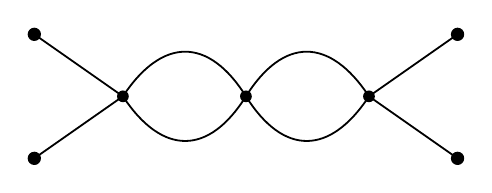
\begin{tikzpicture}[
  x=1.25cm,y=1.05cm,
  line/.style={line width=0.65pt},
  vertex/.style={circle,fill,inner sep=1.5pt},
  endpoint/.style={circle,fill,inner sep=1.7pt}]
  \coordinate (L) at (-1.25,0);
  \coordinate (C) at (0,0);
  \coordinate (R) at (1.25,0);
  \coordinate (LT) at (-2.15,.75);
  \coordinate (LB) at (-2.15,-.75);
  \coordinate (RT) at (2.15,.75);
  \coordinate (RB) at (2.15,-.75);
  \draw[line] (LT)--(L)--(LB) (RT)--(R)--(RB);
  \draw[line] (L) .. controls (-.85,.72) and (-.38,.72) .. (C);
  \draw[line] (L) .. controls (-.85,-.72) and (-.38,-.72) .. (C);
  \draw[line] (C) .. controls (.38,.72) and (.85,.72) .. (R);
  \draw[line] (C) .. controls (.38,-.72) and (.85,-.72) .. (R);
  \node[vertex] at (L) {};
  \node[vertex] at (C) {};
  \node[vertex] at (R) {};
  \node[endpoint] at (LT) {};
  \node[endpoint] at (LB) {};
  \node[endpoint] at (RT) {};
  \node[endpoint] at (RB) {};
\end{tikzpicture}
\end{center}

Using the momentum-space Feynman rules, write the complete contribution of
this diagram, including the overall momentum-conserving delta function, all
four external propagators, all internal propagators, the vertex factors, and
the symmetry factor.  Assign a direction and momentum to every internal
line.  Carry out every momentum integral fixed by a vertex delta function,
but leave the two independent loop integrations unevaluated.

\SupplementaryExercise{7}{The Free Dirac Propagator, Its Residues, and Fermionic Signs}
  {(Adapted from Hong Liu and MIT OpenCourseWare, 8.323 Assignment 9, Problem 2.)}
  {mit-823-s23-ps9-ch6-curated-parent-1}
\begin{enumerate}
\item
Starting from the free Dirac mode expansion and spin sums, show that the
time-ordered contraction of \(\psi_\ell(x)\) with \(\bar\psi_m(y)\) is a
first-order differential operator acting on the scalar Feynman propagator.
Translate the result to the chapter's gamma-matrix convention.
\item
Apply the free Dirac operator to the propagator obtained in S.6.13.
Derive the spinor identity times \(\delta^4(x-y)\), carefully retaining
the contact term produced when the derivative acts on time ordering.
\item
Find the momentum-space factors for contracting
\(\partial_\mu\psi(x)\) with \(\bar\psi(y)\), and \(\psi(x)\) with
\(\partial_\mu\bar\psi(y)\), when momentum flows from \(y\) to \(x\).
Explain the relative sign.
\item
Factor the Dirac propagator denominator into its two energy poles.
Evaluate the numerator at each pole and show that the residues reproduce
the positive-energy \(u\)-spinor and negative-energy \(v\)-spinor
completeness sums.
\item
Derive the minus sign in the \(y^0>x^0\) branch of
\(T\{\psi(x)\bar\psi(y)\}\).  Show that omitting it prevents the two
energy-pole residues from combining into a Lorentz-covariant propagator.
\item
Follow the index contractions around a closed fermion loop with \(n\)
bosonic insertions.  Demonstrate why the matrices form a trace and why
one additional minus sign remains relative to a bosonic loop.
\end{enumerate}

\SupplementaryExercise{8}{The Scalar Pole Prescription}
  {(Inspired by David Tong, Lectures on Quantum Field Theory, Section 2.7.1.)}
  {tong-qft-feynman-rules-2006-curated-parent-1}
Locate the two scalar propagator poles in the complex energy plane under
the chapter's \(-i0\) denominator convention.  Explain how their
displacement implements vacuum boundary conditions rather than retarded
boundary conditions.

\SupplementaryExercise{9}{Five-Particle Scattering in Cubic Scalar Theory}
  {(Adapted from University of Cambridge, Part III, Quantum Field Theory,
  Paper 301, 2024, Question 2.)}
  {cambridge-partiii-2024-paper301-q2-ch6}
Consider a real scalar field in four dimensions with the mostly-plus
Lagrangian
\[
 \mathcal L=-\frac12\partial_\mu\phi\partial^\mu\phi
 -\frac12m^2\phi^2-\frac{g}{3!}\phi^3,
\]
where \(m\) and \(g\) are real and positive.
\begin{enumerate}
\item
What is the mass dimension of \(g\)?  Briefly justify the answer.
\item
State the Feynman rules for this theory.  A brief but clear explanation is
sufficient; a derivation of the rules is not required.
\item
Consider two incoming particles with momenta \(p_1,p_2\) and three outgoing
particles with momenta \(k_i\), \(i=1,2,3\).  Starting from the expression
for the scattering operator in terms of creation and annihilation operators,
relate the corresponding matrix element
\[
 \OutBra{k_1,k_2,k_3}S\InKet{p_1,p_2}
\]
to a time-ordered correlation function.  You may use either LSZ reduction
or the Dyson formula.
\item
Draw every connected tree diagram contributing to this process.  If diagrams
differ only by permutations of external particles, one representative may be
drawn provided all allowed permutations are stated explicitly.
\item
Use the Feynman rules to evaluate the contribution to the scattering matrix
from every connected tree diagram in the preceding part.  Again, a compact
representative expression is acceptable only if all external permutations
and their number are made explicit.
\end{enumerate}

\SupplementaryExercise{10}{Reading a Yukawa Fermion Line Backwards and Crossing a Fermion into an Antifermion}
  {(Inspired by David Tong, Lectures on Quantum Field Theory, Sections 3.4 and 5.7 | David Tong, Lectures on Quantum Field Theory, Sections 3.5 and 5.7.)}
  {tong-qft-feynman-rules-2006-curated-parent-3}
\begin{enumerate}
\item
For scalar emission and absorption by a fermion, write the ordered product
of external spinors, coupling matrices, and propagators by following the
fermion arrow backward.  Verify the ordering explicitly with spinor
indices at two vertices.
\item
Begin with a tree-level Yukawa amplitude having an incoming fermion.
Cross that line to an outgoing antifermion by reversing its momentum and
replacing its wavefunction.  Determine the resulting spinor chain and
state which overall signs are conventional.
\end{enumerate}

\SupplementaryExercise{11}{Exchange of Identical External Fermions}
  {(Inspired by David Tong, Lectures on Quantum Field Theory, Section 5.7.)}
  {tong-qft-feynman-rules-2006-curated-parent-4}
Consider two identical fermions scattering through neutral-scalar
exchange.  Write both connected tree amplitudes and derive their relative
minus sign from the ordering of external creation operators, not from the
geometry of the drawings.

\SupplementaryExercise{12}{Pairings from a Gaussian Generator}
  {(Inspired by Daniel Harlow, Lecture Notes for Physics 8.323, Sections 7.2--7.3.)}
  {harlow-qft1-diagrams-2024-curated-parent-1}
Differentiate a multidimensional Gaussian generating function six times.
Prove that the result is a sum over fifteen pairings and interpret every
inverse quadratic kernel as a propagator line.

\SupplementaryExercise{13}{Symmetry Factors from Diagram Automorphisms}
  {(Adapted from Daniel Harlow, \emph{Lecture Notes for Physics 8.323},
  Section 7.8, Homework Problem 3.)}
  {harlow-qft1-2024-ch6-hw3}
Consider the real scalar theory
\[
 \mathcal L=-\frac12\partial_\mu\phi\partial^\mu\phi
 -\frac12m^2\phi^2-\frac{\lambda}{4!}\phi^4.
\]
Define the symmetry factor \(s_D\) of a diagram \(D\) as the number of its
graph automorphisms, with every external point held fixed.  A self-contracted
propagator may be flipped, parallel propagators may be permuted, and
interaction vertices may be permuted only when all incidences and all fixed
external points are preserved.

The connected part of source Figure 16 contains the following two-point
diagrams.  The factors quoted in its caption, in the displayed order, are
\(s_D=1,2,6,4,4\).  (The full numerator also contains products with vacuum
bubbles; division by the vacuum functional removes those disconnected
components.)

\begin{center}
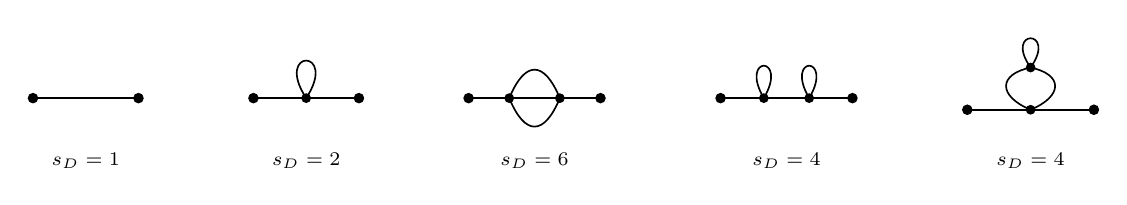
\begin{tikzpicture}[
 x=.67cm,y=.67cm,
 line/.style={line width=.6pt},
 vertex/.style={circle,fill,inner sep=1.25pt},
 endpoint/.style={circle,fill,inner sep=1.35pt},
 every node/.style={font=\scriptsize}]
 % Free line.
 \begin{scope}[xshift=0cm]
  \draw[line] (-1,0)--(1,0);
  \node[endpoint] at (-1,0){}; \node[endpoint] at (1,0){};
  \node at (0,-1.18){\(s_D=1\)};
 \end{scope}
 % One tadpole.
 \begin{scope}[xshift=2.8cm]
  \draw[line] (-1,0)--(1,0);
  \draw[line] (0,0)..controls(-.62,.95)and(.62,.95)..(0,0);
  \node[vertex] at (0,0){};
  \node[endpoint] at (-1,0){}; \node[endpoint] at (1,0){};
  \node at (0,-1.18){\(s_D=2\)};
 \end{scope}
 % Sunset: three parallel internal lines.
 \begin{scope}[xshift=5.7cm]
  \coordinate (a) at (-.48,0); \coordinate (b) at (.48,0);
  \draw[line] (-1.25,0)--(a) (b)--(1.25,0) (a)--(b);
  \draw[line] (a)..controls(-.18,.72)and(.18,.72)..(b);
  \draw[line] (a)..controls(-.18,-.72)and(.18,-.72)..(b);
  \node[vertex] at (a){}; \node[vertex] at (b){};
  \node[endpoint] at (-1.25,0){}; \node[endpoint] at (1.25,0){};
  \node at (0,-1.18){\(s_D=6\)};
 \end{scope}
 % Two tadpoles in series.
 \begin{scope}[xshift=8.9cm]
  \draw[line] (-1.25,0)--(1.25,0);
  \foreach \v in {-.43,.43}{
   \draw[line] (\v,0)..controls(\v-.48,.82)and(\v+.48,.82)..(\v,0);
   \node[vertex] at (\v,0){};
  }
  \node[endpoint] at (-1.25,0){}; \node[endpoint] at (1.25,0){};
  \node at (0,-1.18){\(s_D=4\)};
 \end{scope}
 % Nested tadpole.
 \begin{scope}[xshift=12.0cm]
  \coordinate (a) at (0,-.22); \coordinate (b) at (0,.58);
  \draw[line] (-1.2,-.22)--(a)--(1.2,-.22);
  \draw[line] (a)..controls(-.62,.04)and(-.62,.45)..(b);
  \draw[line] (a)..controls(.62,.04)and(.62,.45)..(b);
  \draw[line] (b)..controls(-.52,1.32)and(.52,1.32)..(b);
  \node[vertex] at (a){}; \node[vertex] at (b){};
  \node[endpoint] at (-1.2,-.22){}; \node[endpoint] at (1.2,-.22){};
  \node at (0,-1.18){\(s_D=4\)};
 \end{scope}
\end{tikzpicture}
\end{center}

For completeness, the disconnected terms drawn in the same source Figure 16
are the free line times one vacuum figure-eight, the free line times two such
vacuum components, the one-tadpole two-point graph times a vacuum
figure-eight, and the free line times each of the two connected two-vertex
vacuum topologies shown below.  These are precisely the terms removed by the
vacuum denominator.

\begin{center}

\begin{tikzpicture}[
 x=.54cm,y=.54cm,
 line/.style={line width=.56pt},
 vertex/.style={circle,fill,inner sep=1.12pt},
 endpoint/.style={circle,fill,inner sep=1.22pt},
 every node/.style={font=\scriptsize}]
 % Free line times a one-vertex vacuum figure-eight.
 \begin{scope}[xshift=0cm]
  \draw[line] (-1.05,.55)--(1.05,.55);
  \node[endpoint] at (-1.05,.55){}; \node[endpoint] at (1.05,.55){};
  \coordinate (v) at (0,-.35);
  \draw[line] (v)..controls(-.52,.35)and(-.52,-1.05)..(v);
  \draw[line] (v)..controls(.52,.35)and(.52,-1.05)..(v);
  \node[vertex] at (v){};
 \end{scope}
 % Free line times two one-vertex vacuum figure-eights.
 \begin{scope}[xshift=3.1cm]
  \draw[line] (-1.05,.65)--(1.05,.65);
  \node[endpoint] at (-1.05,.65){}; \node[endpoint] at (1.05,.65){};
  \foreach \vx in {-.48,.48}{
   \coordinate (v) at (\vx,-.35);
   \draw[line] (v)..controls(\vx-.34,.15)and(\vx-.34,-.85)..(v);
   \draw[line] (v)..controls(\vx+.34,.15)and(\vx+.34,-.85)..(v);
   \node[vertex] at (v){};
  }
 \end{scope}
 % Tadpole two-point graph times a one-vertex vacuum figure-eight.
 \begin{scope}[xshift=6.3cm]
  \draw[line] (-1.05,.58)--(1.05,.58);
  \draw[line] (0,.58)..controls(-.44,1.18)and(.44,1.18)..(0,.58);
  \node[vertex] at (0,.58){};
  \node[endpoint] at (-1.05,.58){}; \node[endpoint] at (1.05,.58){};
  \coordinate (v) at (0,-.4);
  \draw[line] (v)..controls(-.46,.22)and(-.46,-1.02)..(v);
  \draw[line] (v)..controls(.46,.22)and(.46,-1.02)..(v);
  \node[vertex] at (v){};
 \end{scope}
 % Free line times the four-parallel-line vacuum graph.
 \begin{scope}[xshift=9.5cm]
  \draw[line] (-1.05,.7)--(1.05,.7);
  \node[endpoint] at (-1.05,.7){}; \node[endpoint] at (1.05,.7){};
  \coordinate (a) at (-.42,-.35); \coordinate (b) at (.42,-.35);
  \draw[line] (a)--(b);
  \draw[line] (a)..controls(-.18,.1)and(.18,.1)..(b);
  \draw[line] (a)..controls(-.18,-.8)and(.18,-.8)..(b);
  \draw[line] (a)..controls(-.08,-1.12)and(.08,-1.12)..(b);
  \node[vertex] at (a){}; \node[vertex] at (b){};
 \end{scope}
 % Free line times two connected self-loop vertices.
 \begin{scope}[xshift=12.7cm]
  \draw[line] (-1.05,.72)--(1.05,.72);
  \node[endpoint] at (-1.05,.72){}; \node[endpoint] at (1.05,.72){};
  \coordinate (a) at (-.38,-.42); \coordinate (b) at (.38,-.42);
  \draw[line] (a)..controls(-.1,-.05)and(.1,-.05)..(b);
  \draw[line] (a)..controls(-.1,-.78)and(.1,-.78)..(b);
  \draw[line] (a)..controls(-.82,.05)and(-.82,-.88)..(a);
  \draw[line] (b)..controls(.82,.05)and(.82,-.88)..(b);
  \node[vertex] at (a){}; \node[vertex] at (b){};
 \end{scope}
\end{tikzpicture}
\end{center}

Source Figure 18 gives all connected four-point diagrams through order
\(\lambda^2\): the one-vertex tree, four diagrams obtained by inserting a
tadpole on one of its external legs, and the three pairings of the external
points across a pair of vertices joined by two propagators.  Its caption
quotes \(s_D=1\) for the tree and \(s_D=2\) for each of the other seven
diagrams.  The complete topology data are displayed below; the labels on the
last three diagrams record the three partitions of four fixed external
points.

\begin{center}
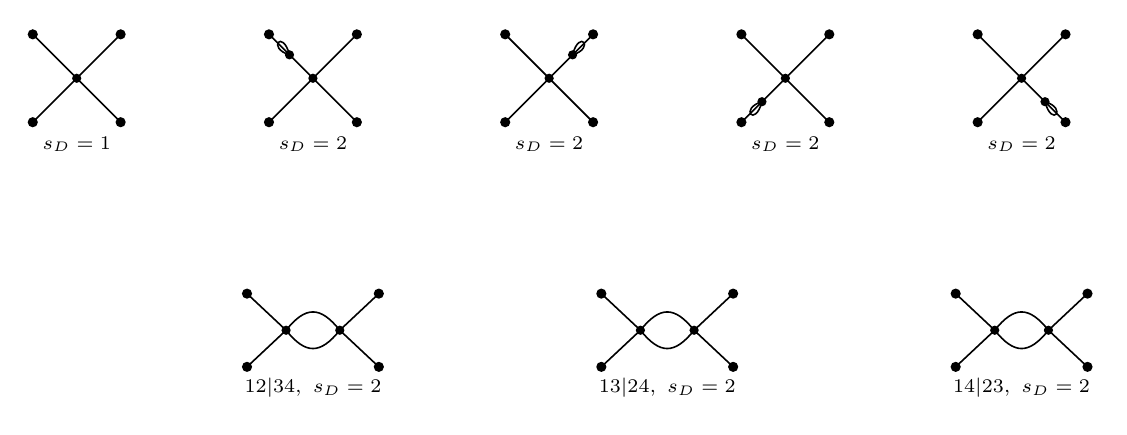
\begin{tikzpicture}[
 x=.62cm,y=.62cm,
 line/.style={line width=.58pt},
 vertex/.style={circle,fill,inner sep=1.18pt},
 endpoint/.style={circle,fill,inner sep=1.3pt},
 every node/.style={font=\scriptsize}]
 % tree and four external-leg tadpoles
 \foreach \sx/\loopleg in {0/0,3/1,6/2,9/3,12/4}{
  \begin{scope}[xshift=\sx cm]
   \coordinate (c) at (0,0);
   \coordinate (nw) at (-.9,.9); \coordinate (ne) at (.9,.9);
   \coordinate (sw) at (-.9,-.9); \coordinate (se) at (.9,-.9);
   \draw[line] (nw)--(c)--(se) (sw)--(c)--(ne);
   \node[vertex] at (c){};
   \node[endpoint] at (nw){}; \node[endpoint] at (ne){};
   \node[endpoint] at (sw){}; \node[endpoint] at (se){};
   \ifnum\loopleg=1
    \coordinate (v) at (-.48,.48);
    \draw[line] (v)..controls(-.95,.62)and(-.62,1.02)..(v); \node[vertex] at (v){};
   \fi
   \ifnum\loopleg=2
    \coordinate (v) at (.48,.48);
    \draw[line] (v)..controls(.62,1.02)and(.95,.62)..(v); \node[vertex] at (v){};
   \fi
   \ifnum\loopleg=3
    \coordinate (v) at (-.48,-.48);
    \draw[line] (v)..controls(-.95,-.62)and(-.62,-1.02)..(v); \node[vertex] at (v){};
   \fi
   \ifnum\loopleg=4
    \coordinate (v) at (.48,-.48);
    \draw[line] (v)..controls(.62,-1.02)and(.95,-.62)..(v); \node[vertex] at (v){};
   \fi
   \ifnum\loopleg=0 \node at (0,-1.35){\(s_D=1\)};
   \else \node at (0,-1.35){\(s_D=2\)}; \fi
  \end{scope}
 }
 % three two-vertex channels
 \foreach \sx/\lab in {3/{12|34},7.5/{13|24},12/{14|23}}{
  \begin{scope}[xshift=\sx cm,yshift=-3.2cm]
   \coordinate (a) at (-.55,0); \coordinate (b) at (.55,0);
   \coordinate (lt) at (-1.35,.75); \coordinate (lb) at (-1.35,-.75);
   \coordinate (rt) at (1.35,.75); \coordinate (rb) at (1.35,-.75);
   \draw[line] (lt)--(a)--(lb) (rt)--(b)--(rb);
   \draw[line] (a)..controls(-.15,.5)and(.15,.5)..(b);
   \draw[line] (a)..controls(-.15,-.5)and(.15,-.5)..(b);
   \node[vertex] at (a){}; \node[vertex] at (b){};
   \node[endpoint] at (lt){}; \node[endpoint] at (lb){};
   \node[endpoint] at (rt){}; \node[endpoint] at (rb){};
   \node at (0,-1.18){\(\lab,\ s_D=2\)};
  \end{scope}
 }
\end{tikzpicture}
\end{center}

Finally, compute rather than assume the symmetry factors of the two diagrams
from source Figure 20:

\begin{center}
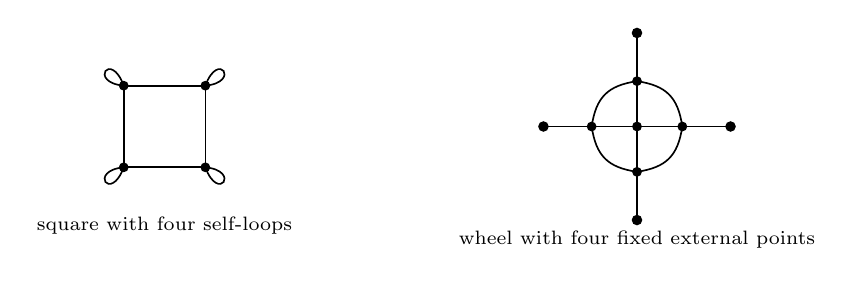
\begin{tikzpicture}[
 x=.72cm,y=.72cm,
 line/.style={line width=.6pt},
 vertex/.style={circle,fill,inner sep=1.25pt},
 endpoint/.style={circle,fill,inner sep=1.35pt},
 every node/.style={font=\scriptsize}]
 % Square vacuum graph with a tadpole at every vertex.
 \begin{scope}[xshift=0cm]
  \coordinate (nw) at (-.72,.72); \coordinate (ne) at (.72,.72);
  \coordinate (sw) at (-.72,-.72); \coordinate (se) at (.72,-.72);
  \draw[line] (nw)--(ne)--(se)--(sw)--cycle;
  \draw[line] (nw)..controls(-1.35,.78)and(-.95,1.35)..(nw);
  \draw[line] (ne)..controls(.95,1.35)and(1.35,.78)..(ne);
  \draw[line] (sw)..controls(-1.35,-.78)and(-.95,-1.35)..(sw);
  \draw[line] (se)..controls(.95,-1.35)and(1.35,-.78)..(se);
  \foreach \v in {nw,ne,sw,se}{\node[vertex] at (\v){};}
  \node at (0,-1.75){square with four self-loops};
 \end{scope}
 % Wheel graph with four fixed external points.
 \begin{scope}[xshift=6.0cm]
  \coordinate (c) at (0,0); \coordinate (n) at (0,.8);
  \coordinate (e) at (.8,0); \coordinate (s) at (0,-.8);
  \coordinate (w) at (-.8,0);
  \draw[line] (n)..controls(.52,.72)and(.72,.52)..(e)
              (e)..controls(.72,-.52)and(.52,-.72)..(s)
              (s)..controls(-.52,-.72)and(-.72,-.52)..(w)
              (w)..controls(-.72,.52)and(-.52,.72)..(n);
  \draw[line] (c)--(n)--(0,1.65) (c)--(e)--(1.65,0)
              (c)--(s)--(0,-1.65) (c)--(w)--(-1.65,0);
  \foreach \v in {c,n,e,s,w}{\node[vertex] at (\v){};}
  \foreach \p in {(0,1.65),(1.65,0),(0,-1.65),(-1.65,0)}{
    \node[endpoint] at \p{};
  }
  \node at (0,-2.0){wheel with four fixed external points};
 \end{scope}
\end{tikzpicture}
\end{center}

Verify every symmetry factor quoted for the Figure 16 and Figure 18
topologies, and determine both Figure 20 factors directly from their
automorphism groups.

\SupplementaryExercise{14}{Connected Diagrams from a Logarithm}
  {(Inspired by Daniel Harlow, Lecture Notes for Physics 8.323, Section 7.4.)}
  {harlow-qft1-diagrams-2024-curated-parent-3}
Let \(Z[J]\) be a perturbative vacuum functional and \(W[J]=\log Z[J]\).
Using the first four source derivatives, prove algebraically that
derivatives of \(W\) generate connected correlation functions rather than
all Wick partitions.

\SupplementaryExercise{15}{Propagator Corrections in a Solvable Theory}
  {(Adapted from John McGreevy, Physics 215A, Fall 2023, Assignment 7,
  Problem 4.)}
  {mcgreevy-215a-f23-hw07-p4-ch6}
Consider a scalar field in \(D\) spacetime dimensions with action
\[
 S=S_0+S_1,
 \qquad
 S_0=-\frac12\int d^Dx\,
   \bigl(\partial_\mu\phi\partial^\mu\phi+m_0^2\phi^2\bigr),
 \qquad
 S_1=-\frac12\int d^Dx\,\delta m^2\phi^2.
\]
The mass term has been artificially split into two pieces.  Perform
perturbation theory in small \(\delta m^2\), treating \(S_1\) as an
interaction, and show that the resulting expansion reassembles the complete
mass.
\begin{enumerate}
\item
Write every Feynman rule for this perturbation theory.
\item
Determine the one-particle-irreducible two-point function, defined by
\[
 -i\Sigma(p)\equiv
 \sum\bigl(\text{all 1PI diagrams with two external nubbins}\bigr).
\]
\item
Geometrically sum all propagator corrections and show that the result is
the propagator one would have written without splitting
\(m_0^2+\delta m^2\).
\end{enumerate}
\end{enumerate}
